% ===========================================================
% 6. EXPERIMENTS
% ===========================================================
\section{Experiments}
\label{sec:experiments}

% Reduce vertical gaps between floats and text
\setlength{\floatsep}{8pt plus 2pt minus 2pt}
\setlength{\textfloatsep}{10pt plus 2pt minus 2pt}
\setlength{\intextsep}{8pt plus 2pt minus 2pt}

\subsection{Simulation Evaluation}
\label{sec:exp-sim}

We evaluate ABot-N1 in simulation across all five core tasks. To
keep the comparison directly interpretable, every task is reported
under the most widely adopted protocol in its respective literature
(VLN-CE R2R/RxR for \textit{instruction-following}, TrackVLA's EVT-Bench for
\textit{person-following}) or under the closed-loop benchmarks introduced in
Sec.~\ref{sec:benchmark} (ABotN-PointBench, ABotN-POIBench, and an
\textit{object-goal} benchmark derived from OVON, defined below). Unless
specified, ``\textbf{ABot-N1}'' refers to the joint multi-task
checkpoint co-trained on all five tasks---our primary model
demonstrating generalist capability and scaling---and
``ABot-N1$^\dagger$'' to the variant fine-tuned on each
individual task, demonstrating the intrinsic framework advantage.
\begin{table}[t]
\centering
\caption{\textbf{Quantitative Instruction-Following Results on the VLN-CE Benchmarks.} Comparison on the VLN-CE Val-Unseen splits of R2R-CE and
RxR-CE. ``S.RGB''\,=\,single-view RGB; ``Pano.''\,=\,panoramic
RGB; ``Depth''/``Odo.'' indicate depth and odometry availability.
Methods marked with $^{\ast}$ use the waypoint predictor
from~\cite{hong2022bridge}.
ABot-N1 achieves the best NE, SR, and SPL on R2R-CE and the best NE on RxR-CE, using only panoramic RGB without depth or odometry.}
\label{tab:exp-vlnce}
\small
\setlength{\tabcolsep}{3pt}
\begin{tabular}{l cccc cccc ccc}
\toprule
 & \multicolumn{4}{c}{\textbf{Observation}} & \multicolumn{4}{c}{\textbf{R2R-CE Val-Unseen}} & \multicolumn{3}{c}{\textbf{RxR-CE Val-Unseen}} \\
\cmidrule(lr){2-5} \cmidrule(lr){6-9} \cmidrule(lr){10-12}
\textbf{Method} & S.RGB & Pano. & Depth & Odo. & NE$\downarrow$ & OSR$\uparrow$ & SR$\uparrow$ & SPL$\uparrow$ & NE$\downarrow$ & SR$\uparrow$ & SPL$\uparrow$ \\
\midrule
HPN+DN$^{\ast}$~\cite{krantz2021waypoint}          &            & \checkmark & \checkmark & \checkmark & 6.31 & 40.0 & 36.0 & 34.0 & --    & --   & --   \\
CMA$^{\ast}$~\cite{hong2022bridge}                 &            & \checkmark & \checkmark & \checkmark & 6.20 & 52.0 & 41.0 & 36.0 & 8.76  & 26.5 & 22.1 \\
Sim2Sim$^{\ast}$~\cite{krantz2022sim2sim}          &            & \checkmark & \checkmark & \checkmark & 6.07 & 52.0 & 43.0 & 36.0 & 8.76  & 26.5 & 22.1 \\
GridMM$^{\ast}$~\cite{wang2023gridmm}              &            & \checkmark & \checkmark & \checkmark & 5.11 & 61.0 & 49.0 & 41.0 & --    & --   & --   \\
DreamWalker$^{\ast}$~\cite{wang2023dreamwalker}    &            & \checkmark & \checkmark & \checkmark & 5.53 & 59.0 & 49.0 & 44.0 & --    & --   & --   \\
Reborn$^{\ast}$~\cite{an2022rxrhabitat}            &            & \checkmark & \checkmark & \checkmark & 5.40 & 57.0 & 50.0 & 46.0 & 5.98  & 48.6 & 42.0 \\
ETPNav$^{\ast}$~\cite{an2024etpnav}                &            & \checkmark & \checkmark & \checkmark & 4.71 & 65.0 & 57.0 & 49.0 & 5.64  & 54.7 & 44.8 \\
HNR$^{\ast}$~\cite{wang2024lookahead}                    &            & \checkmark & \checkmark & \checkmark & 4.42 & 67.0 & 61.0 & 51.0 & 5.50  & 56.3 & 46.7 \\
\midrule
InstructNav~\cite{long2024instructnav}             &            & \checkmark & \checkmark & \checkmark & 6.89 & --   & 31.0 & 24.0 & --    & --   & --   \\
AO-Planner~\cite{chen2025affordances}                &            & \checkmark & \checkmark &            & 5.55 & 59.0 & 47.0 & 33.0 & --    & --   & --   \\
NaVid~\cite{zhang2024navid}                        & \checkmark &            &            &            & 5.47 & 49.0 & 37.0 & 35.0 & --    & --   & --   \\
Uni-NaVid~\cite{zhang2024uninavid}                 & \checkmark &            &            &            & 5.58 & 53.5 & 47.0 & 42.7 & 6.24  & 48.7 & 40.9 \\
NaVILA~\cite{cheng2025navila}                      & \checkmark &            &            &            & 5.22 & 62.5 & 54.0 & 49.0 & 6.77  & 49.3 & 44.0 \\
StreamVLN~\cite{wei2025streamvln}                  & \checkmark &            &            &            & 4.98 & 64.2 & 56.9 & 51.9 & 6.22  & 52.9 & 46.0 \\
CorrectNav~\cite{yu2026correctnav}                & \checkmark &            &            &            & 4.24 & 67.5 & 65.1 & 62.3 & 4.09  & 69.3 & 63.3 \\
NavFoM~\cite{zhang2025navfom}                      &            & \checkmark &            &            & 4.61 & 72.1 & 61.7 & 55.3 & 4.74  & 64.4 & 56.2 \\
NavForesee~\cite{liu2025navforesee}                &            & \checkmark &            &            & 3.94 & \textbf{78.4} & 66.2 & 59.7 & 4.20  & 66.3 & 53.2 \\

Qwen-VLA~\cite{wang2026qwenvla}                    & \checkmark &            &            &            & 5.10 & 69.0 & 57.3 & 51.2 & 5.80  & 59.6 & 47.8 \\
ABot-N0~\cite{abotn0}                              &            & \checkmark &            &            & 3.80 & 70.8 & 66.4 & 63.9 & 3.83 & 69.3 & 60.0 \\
Qwen-RobotNav-4B \cite{zhang2026qwenrobotnav}                    &            & \checkmark &            &            & 3.80 & 77.2 & 69.5 & 63.6 & --            & \textbf{75.2} & \textbf{65.0} \\
\midrule
ABot-N1$^\dagger$            &            & \checkmark &            &            & 3.91 & 71.7 & 68.3 & 66.6 & 3.43    & 70.9   & 61.4   \\
\textbf{ABot-N1}          &            & \checkmark &            &            & \textbf{3.32} & 75.2 & \textbf{70.9} & \textbf{67.5} & \textbf{3.13}     & 73.9   & 63.9   \\
\bottomrule
\end{tabular}
\end{table}

\FloatBarrier
\subsubsection{Instruction-Following: VLN-CE R2R/RxR}
\label{sec:exp-vlnce}

\paragraph{Protocol.}
We evaluate on the Habitat~\cite{savva2019habitat} VLN-CE
Val-Unseen splits of R2R-CE~\cite{krantz2020vlnce} and
RxR-CE~\cite{ku2020rxr}, using standard metrics: navigation
error (NE), oracle success rate (OSR), success rate
(SR), and success weighted by path length (SPL).
Table~\ref{tab:exp-vlnce} categorizes methods to provide a clear
comparison for ABot-N1:
(i)~sensor-heavy methods (top block) using panoramic RGB, depth,
and odometry-based waypoints;
(ii)~recent foundation models and VLMs (middle block) that shift
towards minimal sensor suites, including both single-view (S.RGB)
and panoramic (Pano.) inputs without relying on specialized mapping;
and (iii)~our proposed ABot-N1 (bottom block). Note that 
ABot-N1 takes only a front-left-right tri-view---three
fixed camera views---rather than a dense $360^\circ$ panoramic sweep,
which we categorize under the panoramic (Pano.) column for brevity.


\paragraph{Analysis.}
ABot-N1 sets a new state of the art on R2R-CE Val-Unseen in NE
(3.32\,m), SR (70.89\%), and SPL
(67.5\%), surpassing all baselines---including
depth-and-odometry methods in the top block---while using only a
front-left-right tri-view of RGB. NavForesee retains the highest OSR (78.4\%); ABot-N1
trades marginal OSR for substantially higher SR/SPL, indicating more
decisive goal-reaching rather than merely passing near the target.
On RxR-CE Val-Unseen, ABot-N1 achieves the best NE (\textbf{3.13\,m})
across all reported methods. SR (73.85\%) and SPL (63.85\%) rank second
only to Qwen-RobotNav-4B (75.2\%/65.0\%), which was trained on
significantly larger in-domain RxR data; ABot-N1 nonetheless
outperforms all other methods including CorrectNav (69.3\%/63.3\%)
and NavFoM (64.4\%/56.2\%).
Comparing ABot-N1 with ABot-N1$^\dagger$: the joint multi-task model
matches or exceeds the single-task specialist on both splits (R2R SR
+2.63, RxR SR +2.95), demonstrating that multi-task co-training
yields positive cross-task transfer rather than catastrophic
interference.
We attribute the gain over prior work to two mechanisms: the
affordance pixel re-grounds the slow system's instruction-progress
reasoning into image-space anchors that the fast controller
tracks, and the explicit
``done\,/\,current'' sub-instruction CoT eliminates the
ambiguous mid-segment behavior that single-system VLN policies often
exhibit on long instructions.

\FloatBarrier
\subsubsection{Object-Goal: Short-Horizon OVON}
\label{sec:exp-objgoal}

\paragraph{Protocol.}
As motivated in Sec.~\ref{sec:bench-pointgoal} and the
Introduction, naive long-horizon \textit{object-goal} evaluation conflates
``find the object'' with ``reach the object'', confounding
recognition errors with execution failures. We therefore evaluate
on a re-curated short-horizon OVON benchmark \cite{yokoyama2024hmovon}: starting from the
original OVON Val-Unseen split, we manually annotate the first
frame in which each target object becomes visible across 36
scenes, and re-anchor the start pose to that frame. The resulting
episodes isolate the recognition-and-approach phase, providing a
clean measurement of out-of-vocabulary generalization and
final-meters arrival. We report SR, SPL, and the average
Distance-to-Goal (DTG) at termination.

\begin{table}[t]
\centering
% \caption{\textbf{Quantitative Results on the Short-Horizon OVON Benchmark.}  Object-Goal results on the short-horizon OVON benchmark.
% DTG is the agent--target distance at episode termination (m).
% ABot-N1 substantially improves SR and SPL over all baselines while halving DTG.}
\caption{\textbf{Quantitative Object-Goal Results on the Short-Horizon OVON Benchmark.} 
We report the SR, SPL, and DTG at episode termination. 
Our proposed \textbf{ABot-N1} establishes new state-of-the-art (SOTA) performance by substantially improving both SR and SPL over existing baselines, while successfully halving the final distance-to-goal (DTG).}




\label{tab:exp-objgoal}
\small
\begin{tabular}{lccc}
\toprule
\textbf{Method} & SR$\uparrow$ & SPL$\uparrow$ & DTG$\downarrow$ \\
\midrule
StreamVLN \cite{wei2025streamvln}              & 39.7 & 15.8 & 2.368 \\
NaVILA    \cite{cheng2025navila}             & 55.4 & 26.1 & 1.811 \\
InternVLA-N1 (S2 only) \cite{wei2025ground} & 58.5 & 30.0 & 1.441 \\
Uni-NaVid \cite{zhang2024uninavid}            & 68.7 & 34.5 & 1.495 \\
ABot-N0 \cite{abotn0}               & 73.2 & 35.4 & 1.442 \\
\midrule
ABot-N1$^\dagger$            & \textbf{85.5} & 50.8 & \textbf{0.592} \\
\textbf{ABot-N1}          & 84.9 & \textbf{51.8} & 0.822 \\
\bottomrule
\end{tabular}
\end{table}

\paragraph{Analysis.}
ABot-N1 raises SR by +11.7 points and SPL by +16.4 points over
ABot-N0, while compressing DTG from 1.44\,m to 0.82\,m---a
1.8$\times$ reduction reflecting improved last-meter precision.
The single-task ABot-N1$^\dagger$ pushes SR slightly higher (85.5)
and DTG lower (0.59\,m), demonstrating the framework's raw per-task
capability. ABot-N1 only marginally trails ABot-N1$^\dagger$ in SR
(by 0.6 points) while in fact \emph{exceeding} the specialist on
SPL (51.8 vs.\ 50.8), evidencing strong cross-task transfer rather
than catastrophic interference.
The gap to single-system baselines (Uni-NaVid, NaVILA) widens
most on DTG and SPL, consistent with our hypothesis that
decoupling recognition (object pixel) from approach (affordance
pixel) removes the exploration--arrival entanglement that
bottlenecks monolithic policies on out-of-vocabulary targets.

\FloatBarrier
\subsubsection{Point-Goal: ABotN-PointBench}
\label{sec:exp-pointgoal}

\paragraph{Protocol.}
% We evaluate on ABotN-PointBench (Sec.~\ref{sec:bench-pointgoal})
% in closed-loop rollouts within our in-house 3DGS evaluator,
% separating outdoor and indoor splits and further stratifying each into
% difficulty tiers (outdoor: Low / Medium / High; indoor: Low / High)
% based on path length and environmental complexity.
% Outdoor metrics are SR, SPL, Distance Compliance
% Rate (DCR) and Time Compliance Rate (TCR); the latter two penalize policies
% that reach the goal but cut across vehicle lanes or terminate in
% restricted regions. The outdoor split adopts a relaxed collision
% criterion suited to complex open environments: an episode is deemed
% successful only if the agent arrives with fewer than three collision
% events (SR$_{<3\text{col}}$). This redundant collision budget
% accounts for the slight annotation deviations inherent in the
% large-scale outdoor occupancy maps, preventing minor labeling
% inaccuracies near obstacle boundaries from being mistaken for genuine
% navigation failures. The indoor split adopts a strict collision
% criterion: an episode is deemed successful only if the agent arrives
% with no collision event.
We evaluate on ABotN-PointBench (Sec.~\ref{sec:bench-pointgoal}) in closed-loop rollouts within our in-house 3DGS evaluator, separating outdoor and indoor splits and further stratifying each into difficulty tiers (outdoor: Low / Medium / High; indoor: Low / High) based on path length and environmental complexity. Outdoor metrics are SR and SPL. The outdoor split adopts a relaxed collision criterion suited to complex open environments: an episode is deemed successful only if the agent arrives with fewer than three collision events (SR$_{<3\text{col}}$). This redundant collision budget accounts for the slight annotation deviations inherent in the large-scale outdoor occupancy maps, preventing minor labeling inaccuracies near obstacle boundaries from being mistaken for genuine navigation failures. The indoor split adopts a strict collision criterion: an episode is deemed successful only if the agent arrives with no collision event.

Importantly, the success rate (SR) serves as a holistic indicator that naturally reflects the agent's social compliance over both distance and time. Since a socially non-compliant policy (e.g., one that frequently cuts across vehicle lanes or enters restricted pedestrian zones) inevitably fails to navigate safely, achieving a successful, collision-free arrival inherently ensures that the agent has spent the vast majority of its travel distance and execution time within socially compliant pathways.

% \begin{table}[H]
% \centering
% \caption{Point-Goal results on ABotN-PointBench (outdoor split)
% stratified by difficulty. ABot-N1 achieves the highest SR, SPL, DCR,
% and TCR across all difficulty tiers.}
% \label{tab:exp-pointgoal-out}
% \small
% \setlength{\tabcolsep}{2.5pt}
% \begin{tabular}{l cccc cccc cccc cccc}
% \toprule
%  & \multicolumn{4}{c}{\textbf{SR$_{<3\text{col}}\uparrow$}} & \multicolumn{4}{c}{\textbf{SPL$\uparrow$}} & \multicolumn{4}{c}{\textbf{DCR$\uparrow$}} & \multicolumn{4}{c}{\textbf{TCR$\uparrow$}} \\
% \cmidrule(lr){2-5} \cmidrule(lr){6-9} \cmidrule(lr){10-13} \cmidrule(lr){14-17}
% \textbf{Method} & All & L & M & H & All & L & M & H & All & L & M & H & All & L & M & H \\
% \midrule
% GNM~\cite{shah2023gnm}                & 39.1 & 66.7 & 32.0 & 18.7 & 36.7 & 65.3 & 28.4 & 16.5 & 74.3 & 87.1 & 71.1 & 64.6 & 72.8 & 83.2 & 70.0 & 65.2 \\
% ViNT~\cite{shah2023vint}              & 62.2 & 92.0 & 50.7 & 44.0 & 62.2 & 92.0 & 50.6 & 44.0 & 85.1 & 97.2 & 81.5 & 76.5 & 84.2 & 96.6 & 80.7 & 75.2 \\
% NoMaD~\cite{sridhar2024nomad}         & 56.0 & 90.7 & 45.3 & 32.0 & 55.3 & 90.0 & 45.3 & 31.6 & 78.1 & 97.2 & 73.4 & 63.6 & 77.0 & 95.7 & 72.5 & 62.8 \\
% CityWalker~\cite{liu2025citywalker} & 48.9 & 73.3 & 40.0 & 33.3 & 48.3 & 72.0 & 39.7 & 32.8 & 74.8 & 88.6 & 70.5 & 65.2 & 82.9 & 91.9 & 77.4 & 72.7 \\
% SocialNav~\cite{chen2025socialnav}    & 72.0 & 93.3 & 64.0 & 58.7 & 71.9 & 93.2 & 63.9 & 58.7 & 89.8 & 98.0 & 87.4 & 84.0 & 88.6 & 97.3 & 86.2 & 82.2 \\
% ABot-N0~\cite{abotn0}                 & 77.3 & 94.0 & 74.0 & 64.0 & 77.3 & 94.0 & 74.0 & 64.0 & 77.3 & 94.0 & 73.8 & 64.0 & 89.0 & 96.9 & 88.1 & 82.0 \\
% \midrule
% ABot-N1$^\dagger$                     & 92.0 & \textbf{98.7} & 90.7 & 86.7 & 90.7 & \textbf{96.7} & 89.4 & 85.8 & 91.9 & \textbf{98.5} & 90.6 & 86.6 & 96.1 & \textbf{98.8} & 96.1 & 93.5 \\
% \textbf{ABot-N1}                   & \textbf{92.9} & 96.0 & \textbf{94.7} & \textbf{88.0} & \textbf{91.4} & 95.6 & \textbf{92.3} & \textbf{86.4} & \textbf{92.8} & 95.9 & \textbf{94.5} & \textbf{88.0} & \textbf{96.3} & 97.1 & \textbf{97.2} & \textbf{94.7} \\
% \bottomrule
% \end{tabular}
% \end{table}
\begin{table}[t]
\centering
% \caption{Point-Goal results on ABotN-PointBench (outdoor split)
% stratified by difficulty. ABot-N1 achieves the highest SR and SPL across all difficulty tiers.}
\caption{\textbf{Quantitative Point-Goal Results on the Outdoor Split of ABotN-PointBench.} 
We report the success rate under a redundant collision budget ($\text{SR}_{<3\text{col}}$) and SPL, stratified by difficulty tiers: Low (L), Medium (M), and High (H). 
Our proposed \textbf{ABot-N1} establishes new SOTA performance by consistently securing the highest SR and SPL across all difficulty levels, demonstrating its superior capacity for safe and socially compliant navigation in complex open environments.}



\label{tab:exp-pointgoal-out}
\small
\setlength{\tabcolsep}{6.0pt}
\begin{tabular}{l cccc cccc}
\toprule
 & \multicolumn{4}{c}{\textbf{SR$_{<3\text{col}}\uparrow$}} & \multicolumn{4}{c}{\textbf{SPL$\uparrow$}} \\
\cmidrule(lr){2-5} \cmidrule(lr){6-9}
\textbf{Method} & All & L & M & H & All & L & M & H \\
\midrule
GNM~\cite{shah2023gnm}                & 39.1 & 66.7 & 32.0 & 18.7 & 36.7 & 65.3 & 28.4 & 16.5 \\
ViNT~\cite{shah2023vint}              & 62.2 & 92.0 & 50.7 & 44.0 & 62.2 & 92.0 & 50.6 & 44.0 \\
NoMaD~\cite{sridhar2024nomad}         & 56.0 & 90.7 & 45.3 & 32.0 & 55.7 & 90.0 & 45.3 & 31.6 \\
CityWalker~\cite{liu2025citywalker}   & 48.9 & 73.3 & 40.0 & 33.3 & 48.3 & 72.2 & 39.7 & 32.8 \\
SocialNav~\cite{chen2025socialnav}    & 72.0 & 93.3 & 64.0 & 58.7 & 71.9 & 93.2 & 63.9 & 58.7 \\
ABot-N0~\cite{abotn0}                 & 76.9 & 93.3 & 72.0 & 65.3 & 76.9 & 93.3 & 72.0 & 65.3 \\
\midrule
ABot-N1$^\dagger$                     & 92.0 & \textbf{98.7} & 90.7 & 86.7 & 90.7 & \textbf{96.7} & 89.4 & 85.8 \\
\textbf{ABot-N1}                      & \textbf{92.9} & 96.0 & \textbf{94.7} & \textbf{88.0} & \textbf{91.4} & 95.6 & \textbf{92.3} & \textbf{86.4} \\
\bottomrule
\end{tabular}
\end{table}




% \begin{table}[H]
% \centering
% \caption{Point-Goal results on ABotN-PointBench (indoor split)
% stratified by difficulty. Success requires no collision.
% ABot-N1 achieves the highest overall SR (95.4\%) and TCR (99.1\%).}
% \label{tab:exp-pointgoal-in}
% \small
% \setlength{\tabcolsep}{3pt}
% \begin{tabular}{l ccc ccc ccc ccc}
% \toprule
%  & \multicolumn{3}{c}{\textbf{SR$_{<1\text{col}}\uparrow$}} & \multicolumn{3}{c}{\textbf{SPL$\uparrow$}} & \multicolumn{3}{c}{\textbf{DCR$\uparrow$}} & \multicolumn{3}{c}{\textbf{TCR$\uparrow$}} \\
% \cmidrule(lr){2-4} \cmidrule(lr){5-7} \cmidrule(lr){8-10} \cmidrule(lr){11-13}
% \textbf{Method} & All & L & H & All & L & H & All & L & H & All & L & H \\
% \midrule
% GNM~\cite{shah2023gnm}                & 26.7 & 30.8 & 22.5 & 26.6 & 30.6 & 22.5 & 82.9 & 83.7 & 82.2 & 74.5 & 76.2 & 72.8 \\
% ViNT~\cite{shah2023vint}              & 27.9 & 32.5 & 23.3 & 27.9 & 32.4 & 23.3 & 78.8 & 79.3 & 78.3 & 75.9 & 76.0 & 75.8 \\
% NoMaD~\cite{sridhar2024nomad}         & 20.0 & 20.8 & 19.2 & 19.6 & 20.5 & 18.6 & 77.3 & 77.0 & 77.5 & 74.5 & 74.0 & 75.0 \\
% CityWalker~\cite{liu2025citywalker} & 21.7 & 23.3 & 20.0 & 21.6 & 23.3 & 19.9 & 80.6 & 81.1 & 80.2 & 85.6 & 86.6 & 84.7 \\
% SocialNav~\cite{chen2025socialnav}    & 42.5 & 46.7 & 38.3 & 42.5 & 46.7 & 38.3 & 90.1 & 89.6 & 90.5 & 84.4 & 84.1 & 84.7 \\
% ABot-N0~\cite{abotn0}                 & 89.6 & 91.7 & 87.5 & 85.6 & 87.5 & 83.7 & 89.6 & 91.7 & 87.5 & 99.1 & \textbf{99.5} & 98.8 \\
% \midrule
% ABot-N1$^\dagger$                     & 90.4 & 92.5 & 88.3 & 89.4 & 91.5 & 87.4 & 90.4 & 92.5 & 88.3 & 98.7 & 98.9 & 98.4 \\
% \textbf{ABot-N1}                   & \textbf{95.4} & \textbf{95.0} & \textbf{95.8} & \textbf{93.7} & \textbf{93.3} & \textbf{94.2} & \textbf{95.4} & \textbf{95.0} & \textbf{95.8} & \textbf{99.1} & 98.8 & \textbf{99.4} \\
% \bottomrule
% \end{tabular}
% \end{table}
\begin{table}[t]
\centering
\caption{\textbf{Quantitative Point-Goal Results on the Indoor Split of ABotN-PointBench.} 
We report the success rate under a strict zero-collision criterion ($\text{SR}_{<1\text{col}}$) and SPL, stratified by difficulty tiers: Low (L) and High (H). 
Our proposed \textbf{ABot-N1} establishes new SOTA performance by achieving the highest SR ($95.4\%$) and SPL across all difficulty levels, demonstrating its exceptional safety and precision in constrained indoor environments.}

% \caption{Point-Goal results on ABotN-PointBench (indoor split)
% stratified by difficulty. Success requires no collision.
% ABot-N1 achieves the highest overall SR (95.4\%).}
\label{tab:exp-pointgoal-in}
\small
\setlength{\tabcolsep}{6.0pt}
\begin{tabular}{l ccc ccc}
\toprule
 & \multicolumn{3}{c}{\textbf{SR$_{<1\text{col}}\uparrow$}} & \multicolumn{3}{c}{\textbf{SPL$\uparrow$}} \\
\cmidrule(lr){2-4} \cmidrule(lr){5-7}
\textbf{Method} & All & L & H & All & L & H \\
\midrule
GNM~\cite{shah2023gnm}                & 26.7 & 30.8 & 22.5 & 26.6 & 30.6 & 22.5 \\
ViNT~\cite{shah2023vint}              & 27.9 & 32.5 & 23.3 & 27.9 & 32.4 & 23.3 \\
NoMaD~\cite{sridhar2024nomad}         & 20.0 & 20.8 & 19.2 & 19.6 & 20.5 & 18.6 \\
CityWalker~\cite{liu2025citywalker}   & 21.7 & 23.3 & 20.0 & 21.6 & 23.3 & 19.9 \\
SocialNav~\cite{chen2025socialnav}    & 42.5 & 46.7 & 38.3 & 42.5 & 46.7 & 38.3 \\
ABot-N0~\cite{abotn0}                 & 89.6 & 91.7 & 87.5 & 85.6 & 87.5 & 83.7 \\
\midrule
ABot-N1$^\dagger$                     & 90.4 & 92.5 & 88.3 & 89.4 & 91.5 & 87.4 \\
\textbf{ABot-N1}                      & \textbf{95.4} & \textbf{95.0} & \textbf{95.8} & \textbf{93.7} & \textbf{93.3} & \textbf{94.2} \\
\bottomrule
\end{tabular}
\end{table}

\paragraph{Analysis.}
Outdoor results highlight the structural advantage of the
slow-fast factorization: ABot-N1 reaches 92.9\% overall SR with
strong social compliance, improving over ABot-N0
by +16.0 SR while simultaneously raising compliance performance.
The difficulty-stratified view reveals that the gain is particularly
pronounced on the hardest tier (SR: 88.0 vs.\ 65.3, a +22.7-point
jump), where prior policies---lacking any notion of traversable
regions---simply follow the geometrically shortest path to the goal
coordinate, cutting across vehicle lanes and restricted regions and
thus failing to maintain safety and compliance.
By generating a CoT-guided affordance pixel that re-grounds
navigation onto the nearest traversable pathway at every step,
ABot-N1 recovers safe, compliant trajectories that a metric-only
policy cannot maintain.
ABot-N1$^\dagger$ (92.0\% SR / 90.7\% SPL) already outperforms
all baselines, confirming the framework advantage independent of
multi-task data; the full ABot-N1 further improves all metrics,
especially on Medium and High tiers, suggesting that social-rule
semantics learned via \textit{object-goal} and \textit{POI-goal} supervision transfer
back into \textit{point-goal} compliant behavior.
Indoor performance under the strict no-collision criterion
shows ABot-N1 at 95.4\% SR---a +5.8-point gain over ABot-N0
(89.6\%)---with the improvement concentrated on the High-difficulty
set (95.8 vs.\ 87.5), indicating robust generalization to complex
interior layouts.

\FloatBarrier
\subsubsection{POI-Goal: ABotN-POIBench}
\label{sec:exp-poigoal}

\paragraph{Protocol.}
We evaluate on ABotN-POIBench (Sec.~\ref{sec:bench-poigoal}). The
success criterion is final-meters arrival to the annotated
entrance frame: an episode is successful if the agent terminates
within a 2\,m radius of the entrance (SR$_{<2\mathrm{m}}$). We
additionally report SPL against the A$^{\!*}$ reference
trajectory.

\begin{table}[t]
\centering
% \caption{\textbf{Quantitative POI-Goal results on ABotN-POIBench.}
% ABot-N1 nearly doubles the previous best SR while achieving 68.0\% SPL.}
\caption{\textbf{Quantitative POI-Goal Results on the Urban-Scale ABotN-POIBench.} 
We report the entrance arrival success rate ($\text{SR}_{<2\mathrm{m}}$) and SPL compared against representative baselines. 
Our proposed \textbf{ABot-N1} establishes a new SOTA, boosting the success rate to \textbf{77.3\%} and achieving \textbf{72.6\%} SPL.}

% \caption{\textbf{Quantitative POI-Goal Results on the Urban-Scale ABotN-POIBench.} 
% We report the success rate of final-meters arrival within a 2\,m radius of the annotated target entrance ($\text{SR}_{<2\mathrm{m}}$) and SPL calculated against the optimal A$^{\!*}$ reference trajectory. 
% Our proposed \textbf{ABot-N1} establishes new SOTA performance by nearly doubling the success rate of the previous best baseline (boosting SR to $77.3\%$) while securing an exceptional $72.6\%$ SPL, demonstrating its outstanding capability for long-range target localization and precise entrance arrival.}

\label{tab:exp-poigoal}
\small
\begin{tabular}{lcc}
\toprule
\textbf{Method} & SR$_{<2\mathrm{m}}\uparrow$ & SPL$\uparrow$ \\
\midrule
ViNT \cite{shah2023vint}                        & 19.0 & 18.2 \\
OmniNav (vanilla) \cite{xue2025omninav}           & 23.9 & 22.4 \\
OmniNav (BridgeNav training)\cite{xue2025omninav} & 34.4 & 31.5 \\
ABot-N0   \cite{abotn0}                   & 20.9 & 17.7 \\
POINav~\cite{gong2026poinav} & 42.3 & 40.3 \\
\midrule
ABot-N1$^\dagger$             & 69.9 & 59.8 \\
\textbf{ABot-N1}           & \textbf{77.3} & \textbf{72.6} \\
\bottomrule
\end{tabular}
\end{table}

\paragraph{Analysis.}
ABot-N1 sets a new state of the art on ABotN-POIBench, raising
SR$_{<2\mathrm{m}}$ from 42.3\% (POINav) to 77.3\% (+35.0 points)
and SPL from 40.3\% to 72.6\% (+32.3 points). Even ABot-N1$^\dagger$
variant already achieves 69.9\%\,/\,59.8\%, confirming the framework
advantage alone; the full ABot-N1 pushes further, benefiting from
the largest cross-task synergy we observe: \textit{POI-goal} supervises
only the slow system, so its fast controller benefits from
\textit{point-goal} data, while its slow system benefits from
\textit{object-goal}-style visibility reasoning. The contrast with
OmniNav variants is instructive---OmniNav (BridgeNav training)
improves over the vanilla version by 10 points but plateaus,
consistent with the documented BridgeNav rollout-bias on
large-heading-offset starts; ABot-N1's slow system, trained on
$\sim$3.0\,M tri-view annotations including 0.5\,M hard negatives,
avoids this trajectory bias by construction.

\FloatBarrier
\subsubsection{Person-Following: EVT-Bench}
\label{sec:exp-pf}

\paragraph{Protocol.}
We evaluate \textit{person-following} on the closed-loop
EVT-Bench~\cite{wang2025trackvla} in Habitat, using the
identical protocol as ABot-N0~\cite{abotn0} and
TrackVLA~\cite{wang2025trackvla}: each episode requires
the agent to follow a target person under three difficulty
levels -- Single-Target Tracking (STT, nominal following),
Distracted Tracking (DT, similar-looking pedestrians causing
identity confusion), and Ambiguity Tracking (AT, frequent
severe occlusions). For each scenario we report Success
Rate (SR), Tracking Rate (TR, formerly ``following rate''),
and Collision Rate (CR), all in percent.

\begin{table}[t]
\centering
\caption{\textbf{Quantitative Person-Following Results on EVT-Bench~\cite{wang2025trackvla}.}
SR/TR in \%, higher is better; CR in \%, lower is better. The
symbols $\dagger$ and $\ddagger$ indicate the adoption of
GroundingDINO and the SoM+GPT-4o pipeline, respectively, as in
ABot-N0~\cite{abotn0}.
ABot-N1 achieves the best SR and TR across the three splits with the sole exception of STT TR, surpassing ABot-N0 and all baselines.}
\label{tab:exp-pf}
\setlength{\tabcolsep}{3pt}
\small
\begin{tabular}{l ccc ccc ccc}
\toprule
 & \multicolumn{3}{c}{\textbf{Single-Target (STT)}} & \multicolumn{3}{c}{\textbf{Distracted (DT)}} & \multicolumn{3}{c}{\textbf{Ambiguity (AT)}} \\
\cmidrule(lr){2-4} \cmidrule(lr){5-7} \cmidrule(lr){8-10}
\textbf{Method} & SR$\uparrow$ & TR$\uparrow$ & CR$\downarrow$ & SR$\uparrow$ & TR$\uparrow$ & CR$\downarrow$ & SR$\uparrow$ & TR$\uparrow$ & CR$\downarrow$ \\
\midrule
IBVS$^{\ddagger}$~\cite{gupta2016novel}    & 42.9 & 56.2 & 3.75 & 10.6 & 28.4 & 6.14 & 15.2 & 39.5 & \textbf{4.90} \\
PoliFormer$^{\dagger}$~\cite{zeng2024poliformer} & 4.67 & 15.5 & 40.1 & 2.62 & 13.2 & 44.5 & 3.04 & 15.4 & 41.5 \\
EVT$^{\ddagger}$~\cite{zhong2024empowering}      & 32.5 & 49.9 & 40.5 & 15.7 & 35.7 & 53.3 & 18.3 & 21.0 & 44.9 \\
Uni-NaVid~\cite{zhang2024uninavid}            & 25.7 & 39.5 & 41.9 & 11.3 & 27.4 & 43.5 & 8.26 & 28.6 & 43.7 \\
NavFoM~\cite{zhang2025navfom}                 & 85.0 & 80.5 & --   & 61.4 & 68.2 & --   & --   & --   & --   \\
TrackVLA++~\cite{wang2025trackvlapp}          & 86.0 & 81.0 & \textbf{2.10} & 66.5 & 68.8 & \textbf{4.71} & 51.2 & 63.4 & 15.9 \\
Qwen-RobotNav-4B~\cite{zhang2026qwenrobotnav}                              & 77.4 & \textbf{90.0} & 6.40 & --   & --   & --   & --   & --   & --   \\
Qwen-RobotNav-8B~\cite{zhang2026qwenrobotnav}                                & 78.6 & 89.7 & 5.70 & --   & --   & --   & --   & --   & --   \\
ABot-N0~\cite{abotn0}                         & 86.9 & 87.6 & 8.54 & 66.7 & 75.4 & 11.6 & 67.3 & 79.5 & 7.05 \\
\midrule
ABot-N1$^\dagger$                      & 87.0 & 86.9 & 6.83 & 65.2 & 72.7 & 14.7 & \textbf{70.3} & 81.1 & 9.47 \\
\textbf{ABot-N1}                       & \textbf{90.1} & 89.8 & 4.27 & \textbf{67.4} & \textbf{84.4} & 17.9 & 70.0 & \textbf{87.8} & 17.9 \\
\bottomrule
\end{tabular}
\end{table}

\paragraph{Analysis.}
ABot-N1 leads on all SR metrics and on TR for the DT and AT
splits, while matching the top STT TR within 0.2 points. On the easy STT setting, it reaches 90.1 SR /
89.8 TR---surpassing ABot-N0 by +3.2 SR and +2.2 TR while
maintaining comparable CR (4.27 vs.\ 8.54). On the hardest AT split,
ABot-N1 achieves 70.0 SR / 87.8 TR,
improving over ABot-N0 by +2.7 SR and +8.3 TR, confirming that the
asymmetric pixel protocol (target-pixel set to null while the
affordance pixel falls back to the first projectable future waypoint,
cf.\ Sec.~\ref{sec:data-tasks}) effectively hardens re-identification
across severe occlusions. The most striking gain appears on DT, where
ABot-N1 raises TR from 75.4 to 84.4 (+9.0 points) and
SR from 66.7 to 67.4, indicating that joint multi-task
training strengthens the slow system's identity reasoning even
under distractor interference.
The trade-off is a slightly higher CR on DT/AT (17.9\% vs.\ 11.6\%
/ 7.05\%), reflecting a more aggressive approach policy learned from
the combined training set; future work may mitigate this via an explicit collision-avoidance reward during post-training.

\FloatBarrier
\subsubsection{Cross-Task Summary}
\label{sec:exp-summary}

Across the five tasks evaluated in this report,
ABot-N1 improves over ABot-N0 on the primary metric of
every task: +3.9 SR on R2R-CE,
+16.0 SR on ABotN-PointBench (outdoor split) with simultaneously improved
compliance, +0.558 absolute jump in SR$_{<2\mathrm{m}}$ on
ABotN-POIBench, and +3.2 STT-SR / +2.7 AT-SR on EVT-Bench
Person-Following. On short-horizon OVON, ABot-N1$^\dagger$
variant lifts SR by +12.3, confirming the framework advantage
even without multi-task data.
ABot-N1 matches or exceeds ABot-N1$^\dagger$
on \textit{point-goal}, \textit{instruction-following}, and \textit{POI-goal} and only
marginally trails on \textit{object-goal}, indicating that the
unified pixel-goal interface supports positive cross-task
transfer and effective scaling rather than the destructive
interference often reported when training generalist navigators
on heterogeneous data.

\subsection{Real-World Deployment}
\label{sec:exp-real}

To validate the practical applicability of the proposed system, we deploy
the complete ABot-N1 on our proprietary AMap TuTu
quadrupedal robot platform and conduct extensive real-world experiments
in diverse indoor and outdoor environments.

\subsubsection{Hardware Setting}
\label{sec:exp-hw}

The experimental platform is \textbf{AMap TuTu}, a 12-DOF quadrupedal robot equipped with omnidirectional LiDAR, RTK-GNSS, and a Tri-Camera array spanning $270^{\circ}$ horizontal FOV for egocentric perception. 
For ABot-N1, we introduce two key upgrades.
First, we deeply integrate the previously modular perception stack (BEV occupancy mapping, legged odometry, and obstacle filtering) with the VLN inference pipeline into a single unified onboard
framework, eliminating inter-process communication overhead and
reducing end-to-end latency.
Second, we upgrade the compute module from Jetson Orin NX to
Jetson AGX Orin 64\,GB. The $4\times$ memory
expansion and increased GPU throughput are critical for hosting the
dual slow-fast VLN inference concurrently with real-time BEV
perception and locomotion control, enabling the full
navigation architecture to run entirely on-robot without offloading.

\subsubsection{Edge Deployment Scheme}
\label{sec:exp-deploy}

For real-time execution on the edge device, we deploy the full
slow-fast pipeline at an overall control frequency of 10\,Hz.
To ensure robust performance under limited computational resources,
a lightweight model structure together with an asynchronized
sequential execution scheme are deliberately designed as follows.

To reduce parameter size, the slow system is built upon
Qwen-3.5-2B, while the fast system is implemented by a DiT with
306\,M parameters whose visual observations are encoded by a
DINOv2-Base encoder. The two systems operate asynchronously: the
slow system runs at a lower frequency than the fast system, whereas
the fast system runs continuously with cached information from the
slow system and current observations over multiple control cycles.
Once the slow system produces an updated plan, the fast system
generates waypoints conditioned on the latest reasoning result.
This decoupled scheduling maximizes GPU utilization on the Jetson AGX Orin
while maintaining consistent 10\,Hz closed-loop responsiveness.

% TODO: Qualitative visualization, CoT visualization.
% TODO: Experiments: Instruction-Following, indoor/outdoor point-goal,
%       person-following, POI-goal, object-goal.

\subsubsection{Deployment Results}
\label{sec:exp-results}

We present qualitative deployment results across the five core tasks,
demonstrating ABot-N1's real-world reasoning and control capabilities
through representative episodes with slow-system CoT and pixel-level
prediction visualizations.
\begin{figure}[!t]
\centering
% 
\includegraphics[width=\linewidth]{figs/point_exp.pdf}
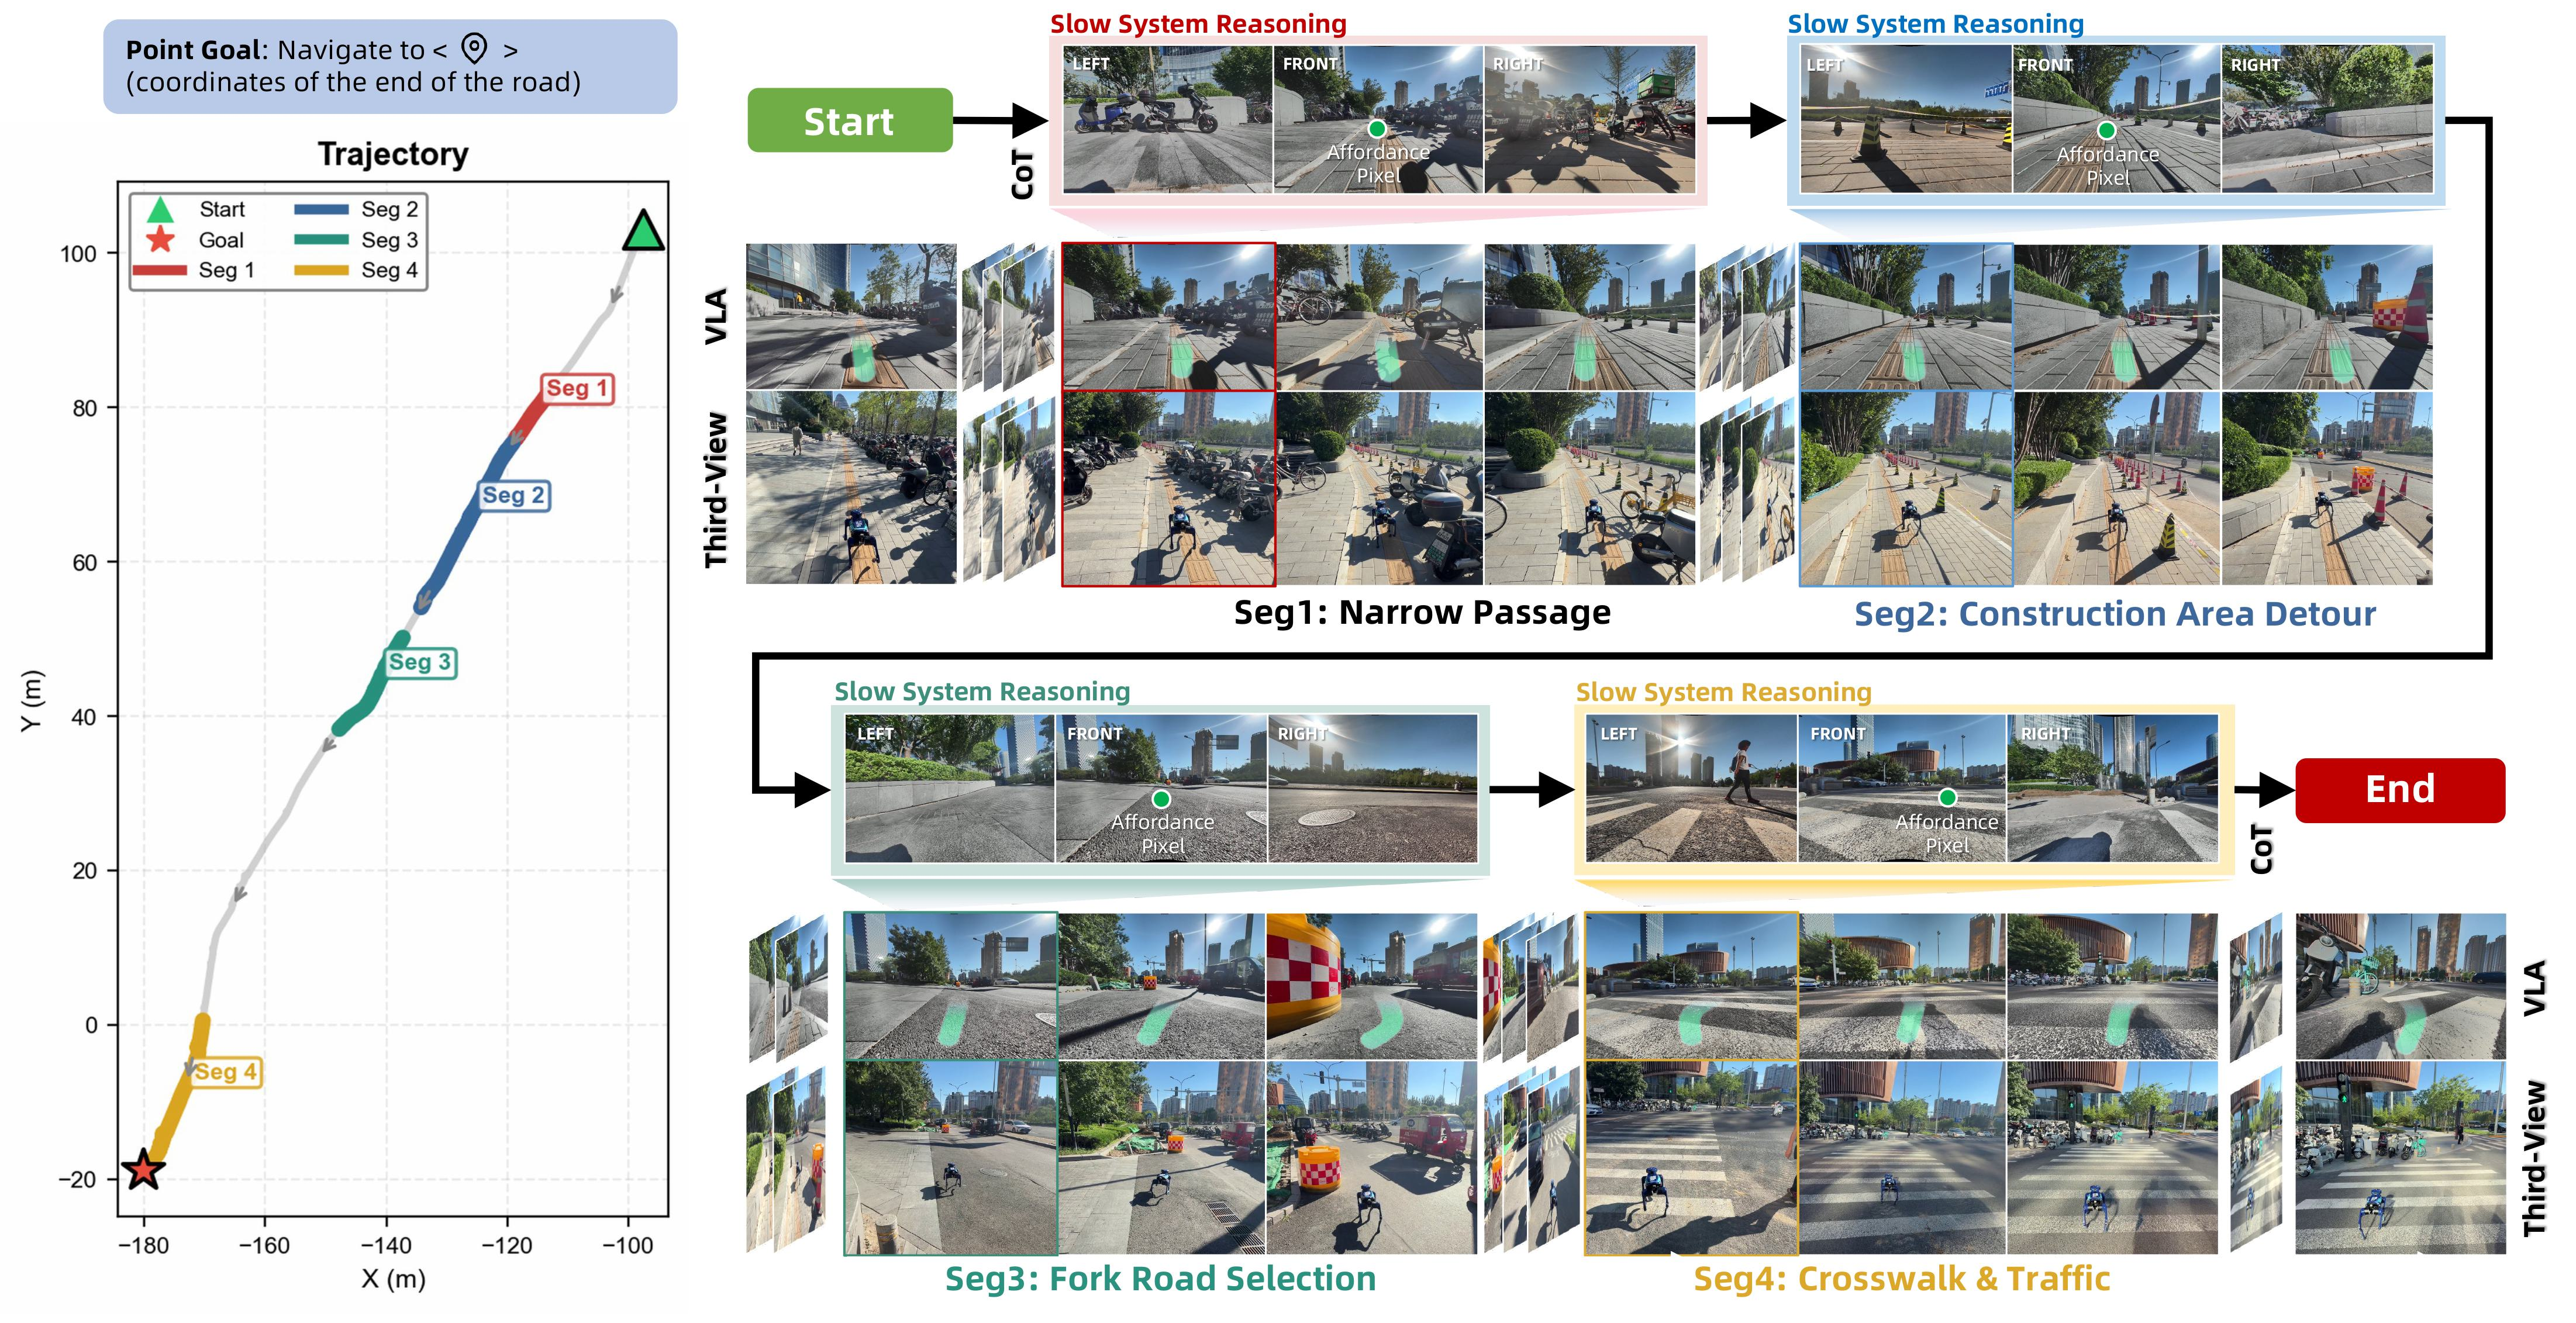
\includegraphics[width=\linewidth]{figs_jpg/point_exp.jpg}
\caption{\textbf{Point-Goal Deployment.} Four segments of a long-range outdoor
episode showcasing obstacle avoidance on narrow roads, construction area detour, correct fork selection, and traffic-light-compliant crosswalk
traversal.}
\label{fig:exp-point}
\end{figure}

\paragraph{Point-Goal Navigation.}
Figure~\ref{fig:exp-point} illustrates a long-distance outdoor
navigation episode decomposed into four representative segments.
(1)~\emph{Narrow-road obstacle avoidance}: the agent successfully
navigates around parked vehicles on a constricted roadway, with the
affordance pixel consistently anchored to the traversable lane.
(2)~\emph{Construction-zone detour}: upon detecting a
construction area, the slow system places the affordance pixel on a
detour around the restricted region, steering the fast controller
clear of the illegal construction zone rather than entering it.
(3)~\emph{Fork selection}: at a road bifurcation, the affordance pixel
is anchored to the target-aligned branch, steering
the agent onto the correct path and avoiding wrong-turn failures.
(4)~\emph{Traffic-light compliance}: approaching a signalized
crosswalk, the agent waits for the green signal before crossing,
demonstrating awareness of traffic rules and the ability to
temporally gate its own actions---a behavior absent from
metric-only \textit{point-goal} policies.
These results confirm that the slow system's traversability-aware
pixel guidance translates into safe, rule-compliant outdoor navigation
beyond simple goal-reaching.

\paragraph{Object-Goal Navigation.}
Figure~\ref{fig:exp-obj} presents three representative \textit{object-goal}
episodes with CoT, affordance pixel, and target pixel outputs.
(1)~\emph{Outdoor bench finding}: the agent locates a park bench
under dappled tree shade at a considerable distance, demonstrating
robust long-range recognition under complex natural lighting.
(2)~\emph{Indoor chair with water bottle}: the slow system reasons
about spatial relations between objects---distinguishing the target
chair \emph{with a water bottle} from other chairs---evidencing
spatial reasoning and attribute-aware recognition.
(3)~\emph{Indoor fire extinguisher}: the agent navigates around
indoor obstacles and identifies a partially occluded fire
extinguisher, showcasing perception under occlusion.
Across all cases, the affordance pixel consistently falls on safe
traversable surfaces while the target pixel locks onto the
goal object once visible, validating the decoupled
recognition-and-approach protocol.

\FloatBarrier

\begin{figure}[!t]
\centering
% 
\includegraphics[width=\linewidth]{figs/obj_exp.pdf}
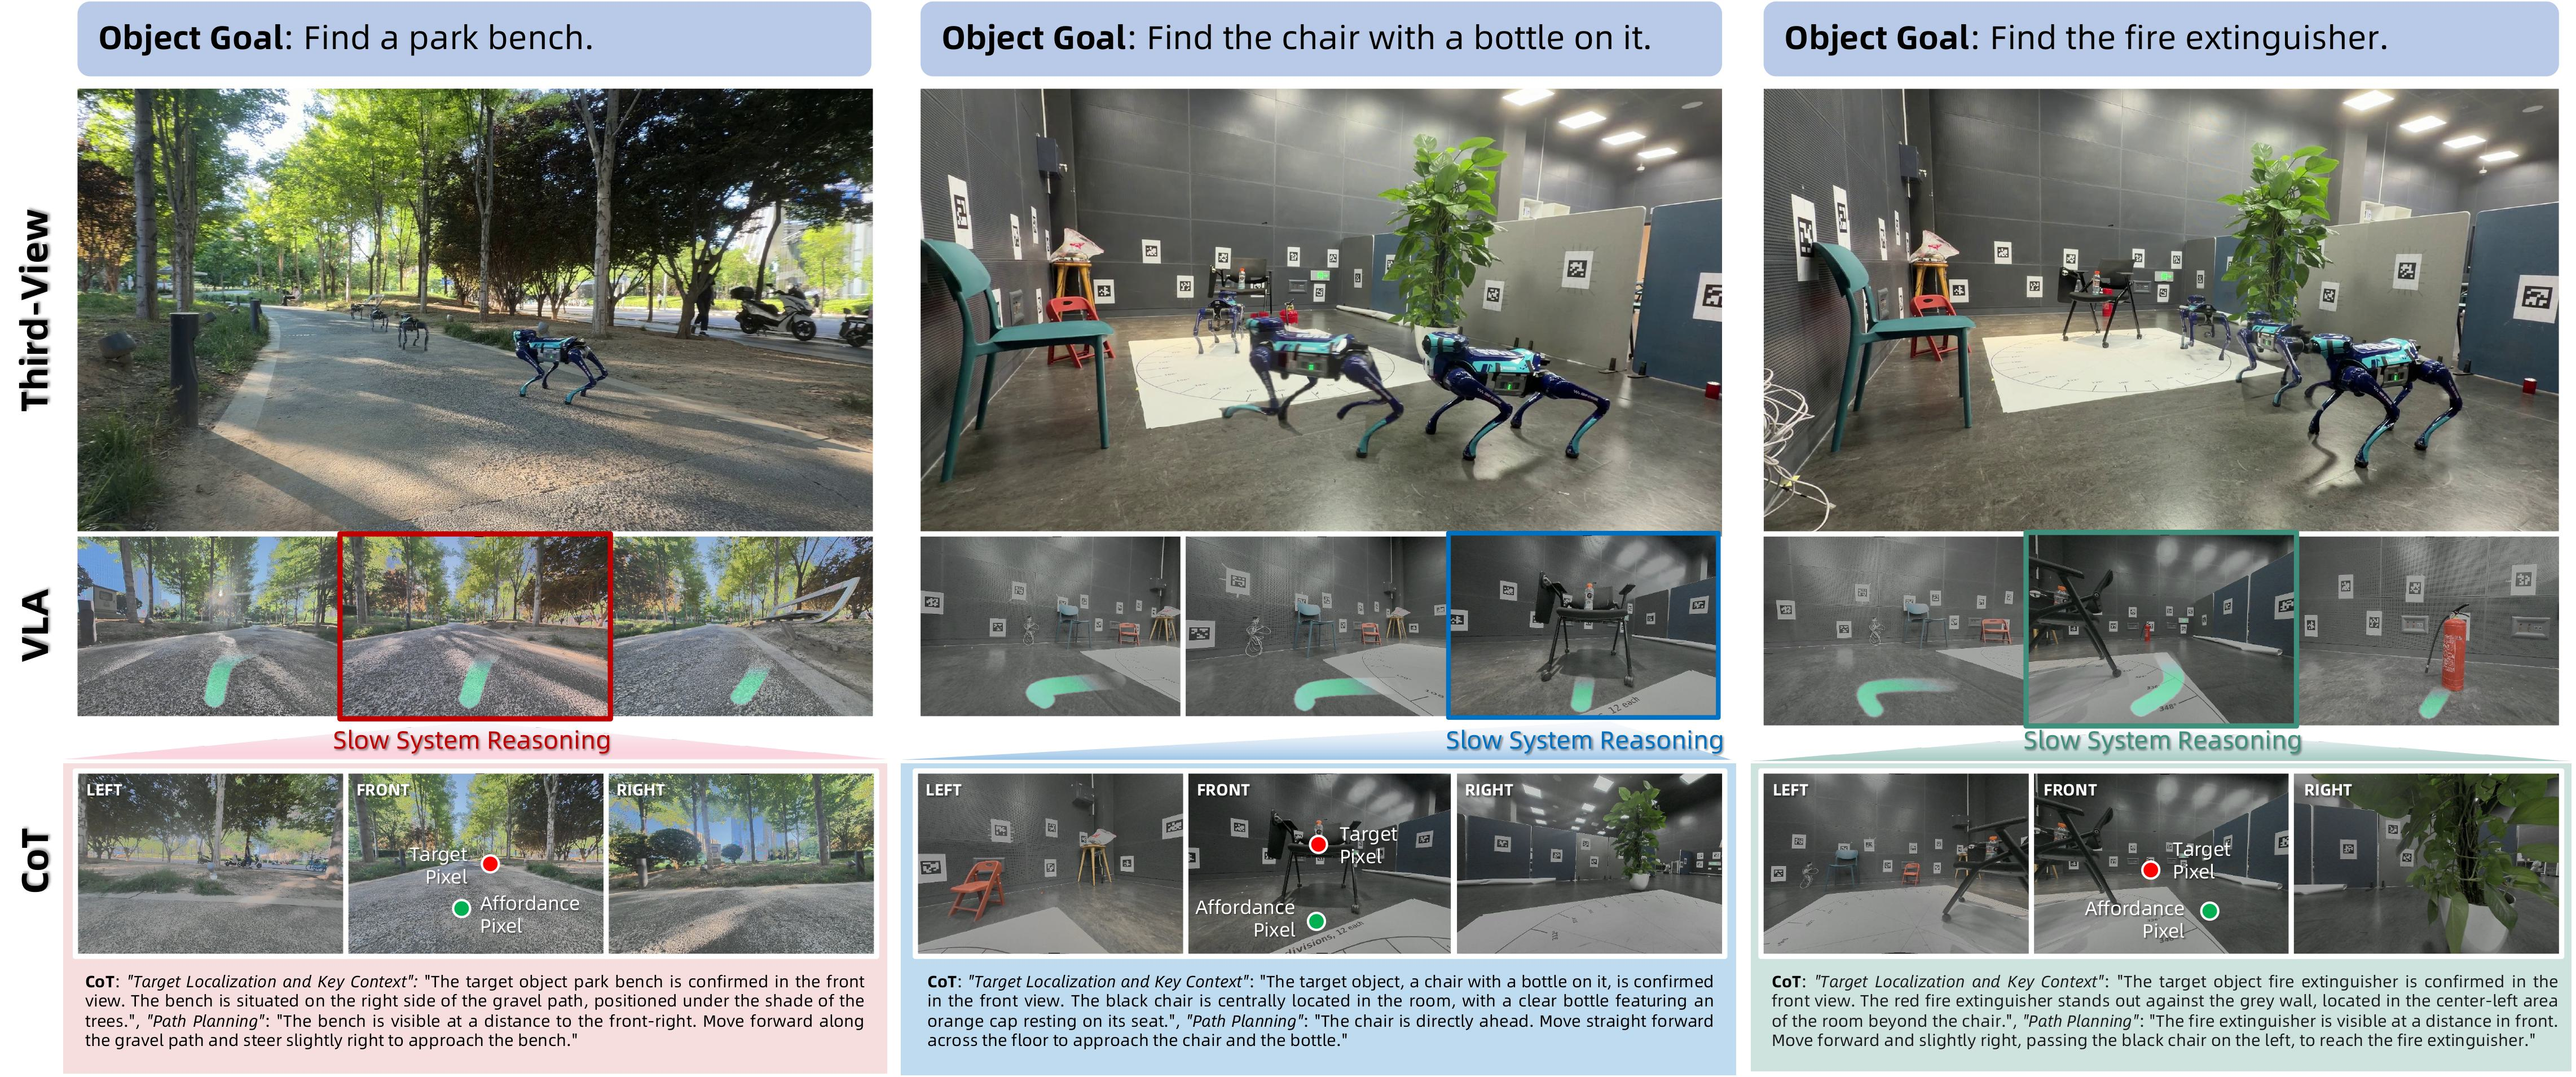
\includegraphics[width=\linewidth]{figs_jpg/obj_exp.jpg}

\caption{\textbf{Object-Goal Deployment.} Three cases---outdoor bench under
dappled tree shade at long range, indoor chair with a water bottle
(spatial reasoning), and partially occluded fire extinguisher---with
CoT, affordance, and target pixel overlays.}
\label{fig:exp-obj}
\end{figure}


\FloatBarrier
\paragraph{POI-Goal Navigation.}
Figure~\ref{fig:exp-poi} shows three \textit{POI-goal} episodes in which
the agent locates commercial storefronts by recognizing signage.
(1)~\emph{Lanzhou beef noodle restaurant}: the agent identifies
the shop sign at a large oblique viewing angle, demonstrating
robust text and logo recognition under perspective distortion.
(2)~\emph{McDonald's}: building upon recognition, the agent
performs obstacle avoidance during approach, coordinating the
affordance pixel around street-level obstructions.
(3)~\emph{Luckin Coffee}: the agent navigates a gentle slope,
identifies a passable entrance, and avoids an impassable staircase
with high steps, demonstrating the slow system's joint reasoning
over accessibility and goal identity.
These results highlight that \textit{POI-goal} requires not only
fine-grained visual recognition but also path-feasibility reasoning,
both of which are naturally captured by the target pixel + affordance pixel
protocol.

\begin{figure}[!t]
\centering
% 
\includegraphics[width=\linewidth]{figs/poi_exp.pdf}
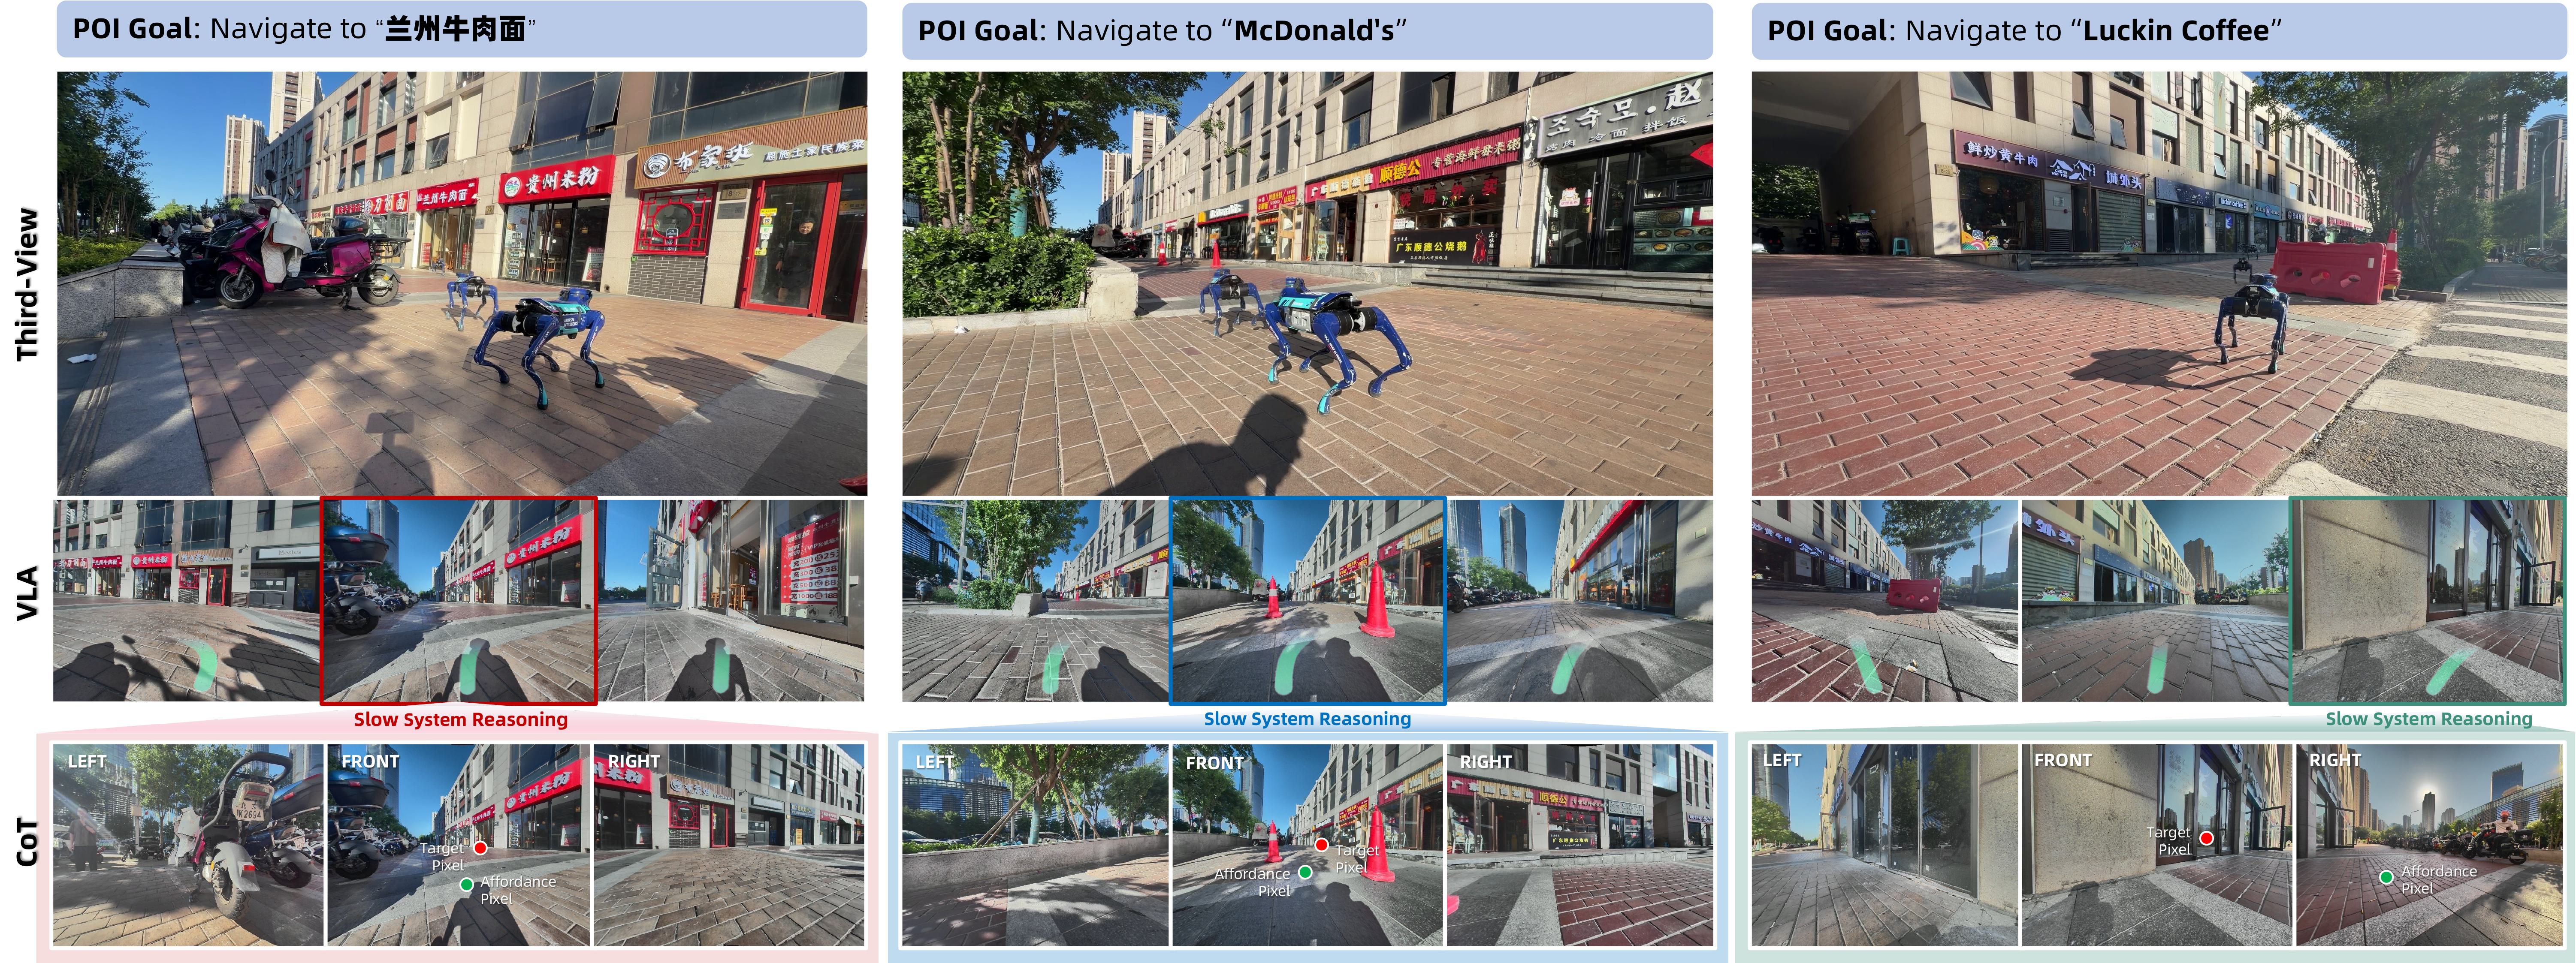
\includegraphics[width=\linewidth]{figs_jpg/poi_exp.jpg}

\caption{\textbf{POI-Goal Deployment.} Locating a Lanzhou noodle restaurant
(large viewing angle), McDonald's (obstacle avoidance en route),
and Luckin Coffee (slope navigation and staircase avoidance).}
\label{fig:exp-poi}
\end{figure}


\FloatBarrier
\paragraph{Instruction-Following.}
Figure~\ref{fig:exp-ins} visualizes four key decision moments
during an indoor \textit{instruction-following} episode with the command:
\emph{``Walk down the stairs \ldots\ approach and stop directly in
front of the bar counter.''}  At each moment the slow system
produces a CoT trace and an affordance pixel (and, near the
destination, a target pixel):
(1)~\emph{Descending stairs}: the CoT identifies the current
sub-instruction and the affordance pixel marks the stairwell path.
(2)~\emph{Entering the gym room}: the reasoning correctly advances
the instruction pointer and anchors the pixel to the gym doorway.
(3)~\emph{Exiting the gym}: the CoT tracks cumulative progress and
shifts the pixel toward the hall exit.
(4)~\emph{Approaching the bar counter}: having recognized the
final landmark, the system emits a target pixel directly on the bar
and prepares to terminate.
The explicit CoT decomposes the long instruction into manageable
sub-goals at each step, eliminating the ambiguous mid-segment
behavior typical of single-system VLN policies.

\begin{figure}[!t]
\centering
% 
\includegraphics[width=\linewidth]{figs/ins_exp.pdf}
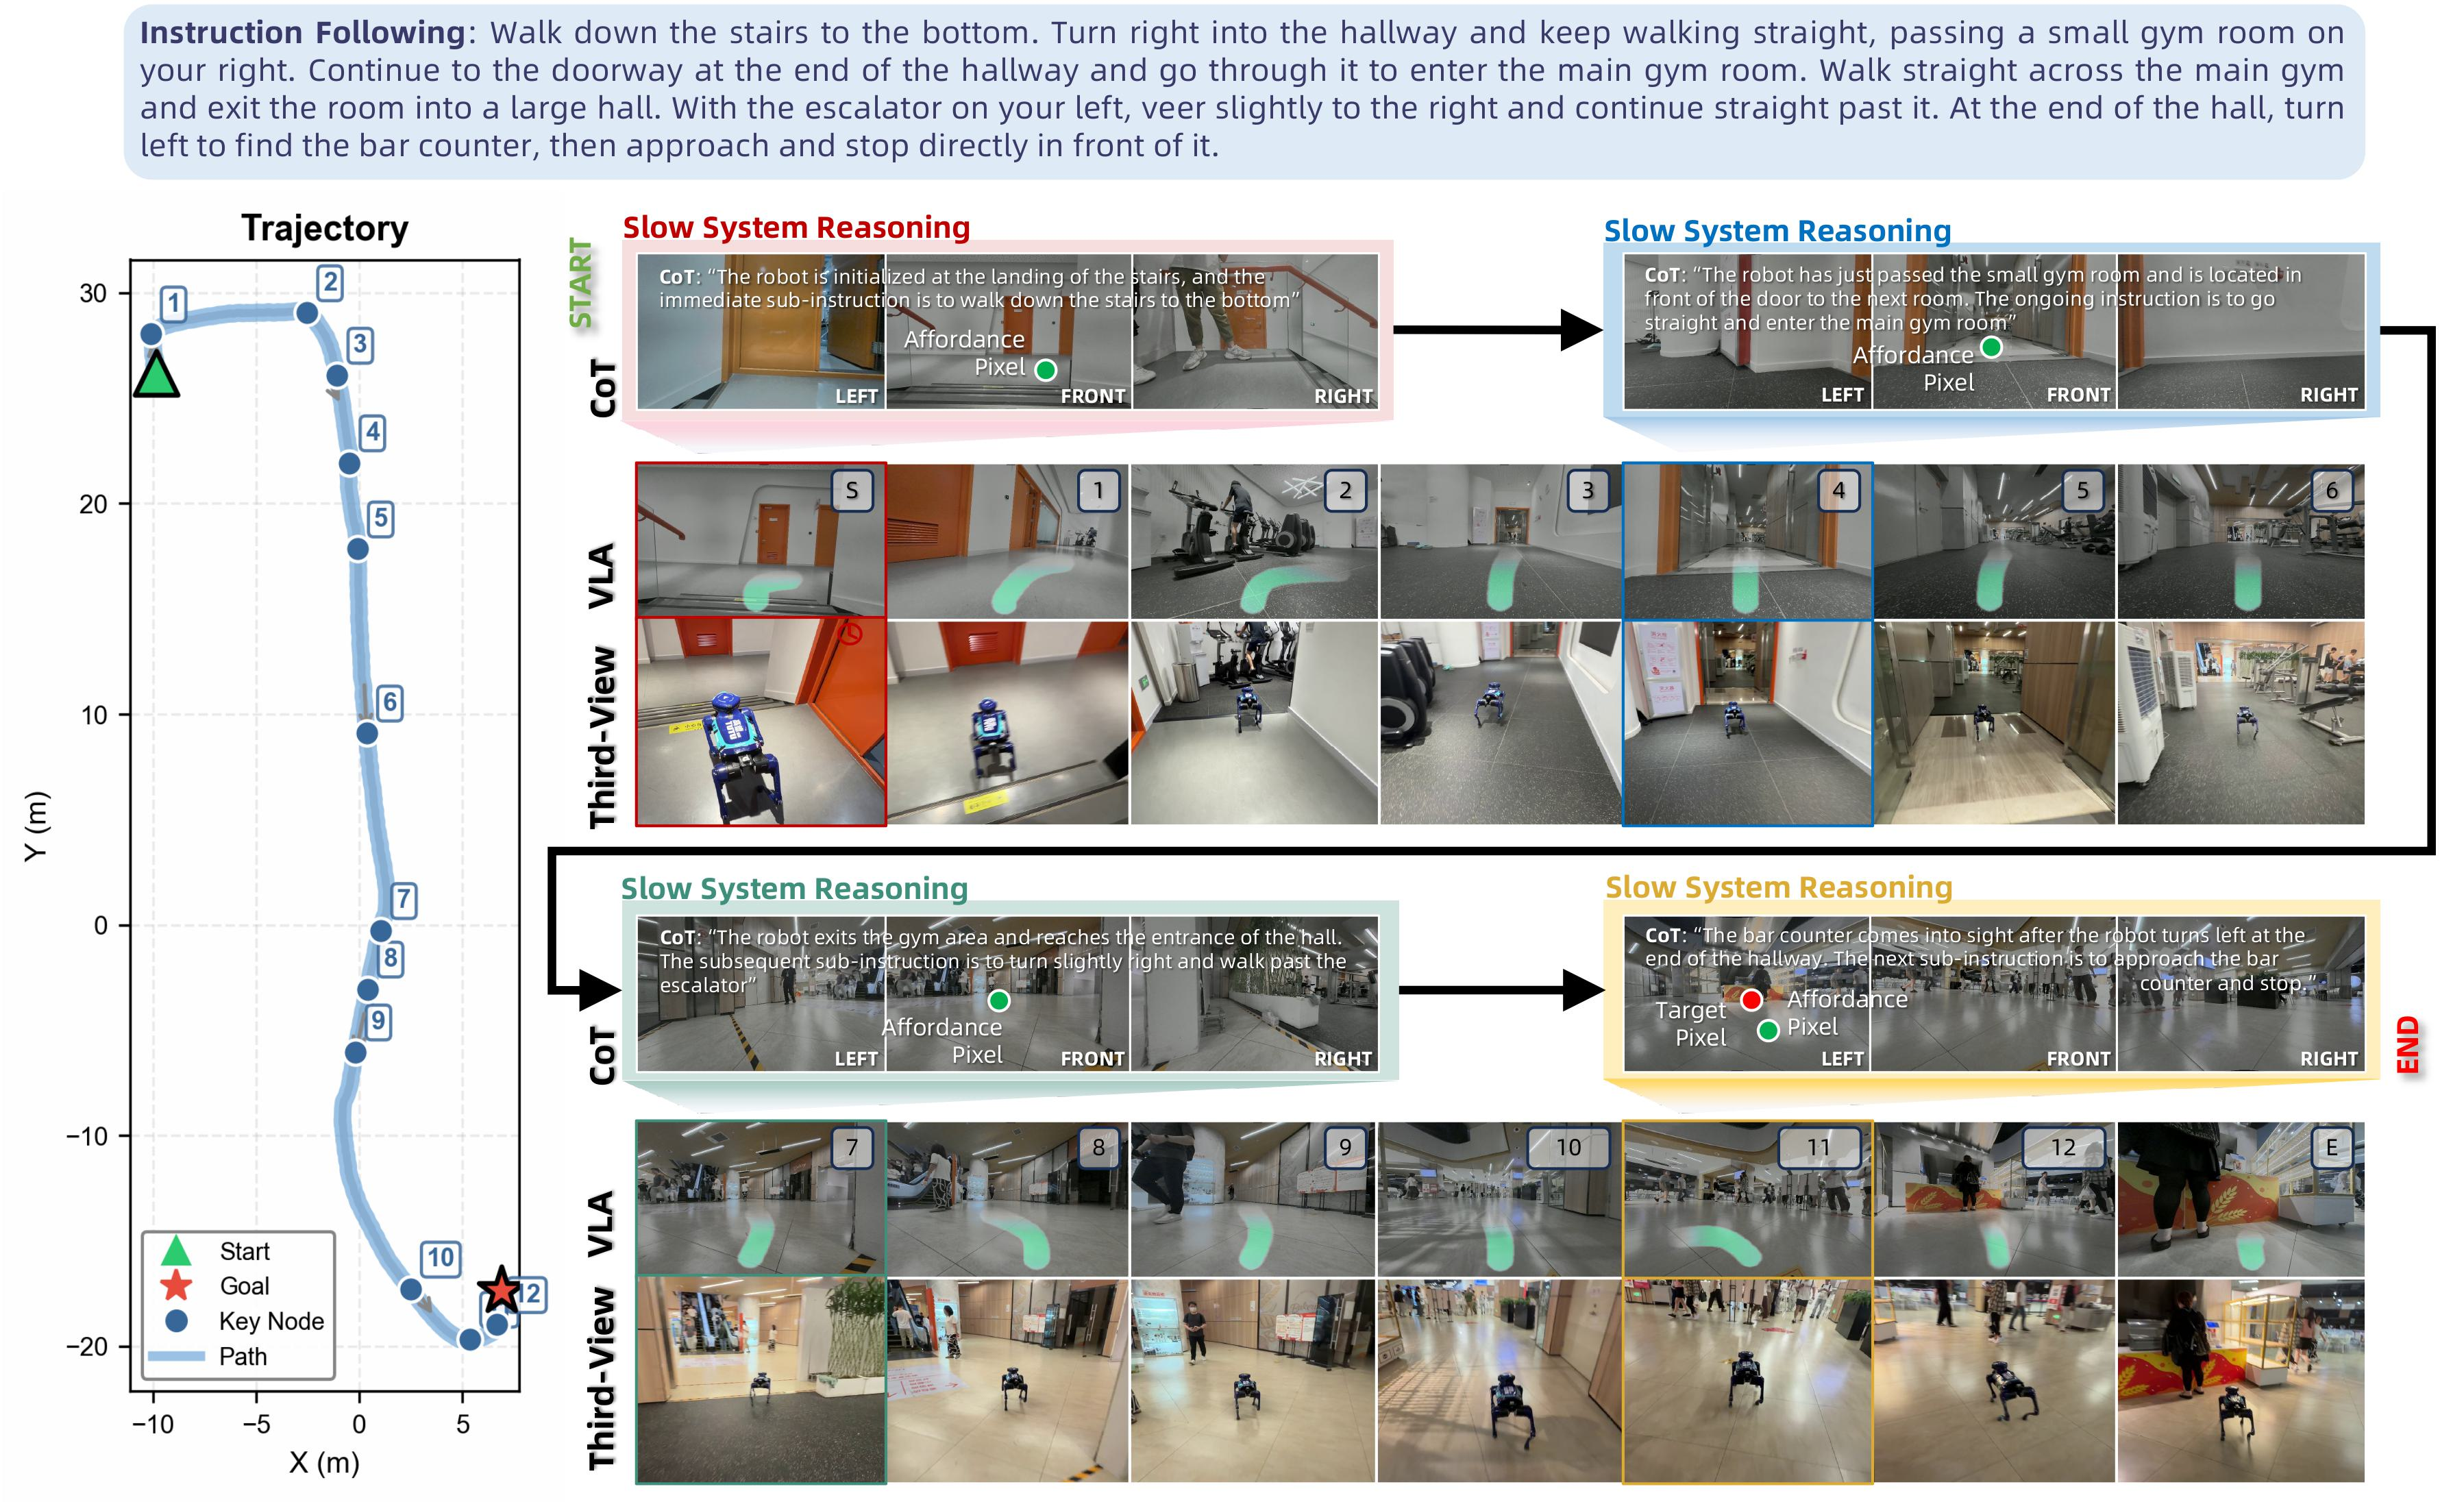
\includegraphics[width=\linewidth]{figs_jpg/ins_exp.jpg}

\caption{ \textbf{Instruction-Following Deployment.} Slow-system reasoning at
four critical moments---stair descent, gym entry, gym exit, and bar
approach---with CoT, affordance pixel, and target pixel
visualizations.}
\label{fig:exp-ins}
\end{figure}

\FloatBarrier
\paragraph{Person-Following.}
Figure~\ref{fig:exp-person} illustrates three Person-Following cases.
(1)~\emph{Outdoor following with distractors}: the agent maintains
stable tracking of the designated target despite the presence of
other pedestrians, demonstrating the slow system's robust identity
reasoning and re-identification capability.
(2)~\emph{Outdoor stair-climbing}: the target ascends a staircase
and the agent follows seamlessly, confirming the fast system's
stable low-level control under elevation changes.
(3)~\emph{Indoor corner tracking}: as the target rounds a sharp
indoor corner, the agent adjusts its heading in time and follows
smoothly while keeping the target continuously in view.
The combination of slow-system identity persistence and
fast-system reactive control ensures continuous, collision-aware
following across challenging real-world conditions.


\begin{figure}[!t]
\centering
% 
\includegraphics[width=\linewidth]{figs/person_exp.pdf}
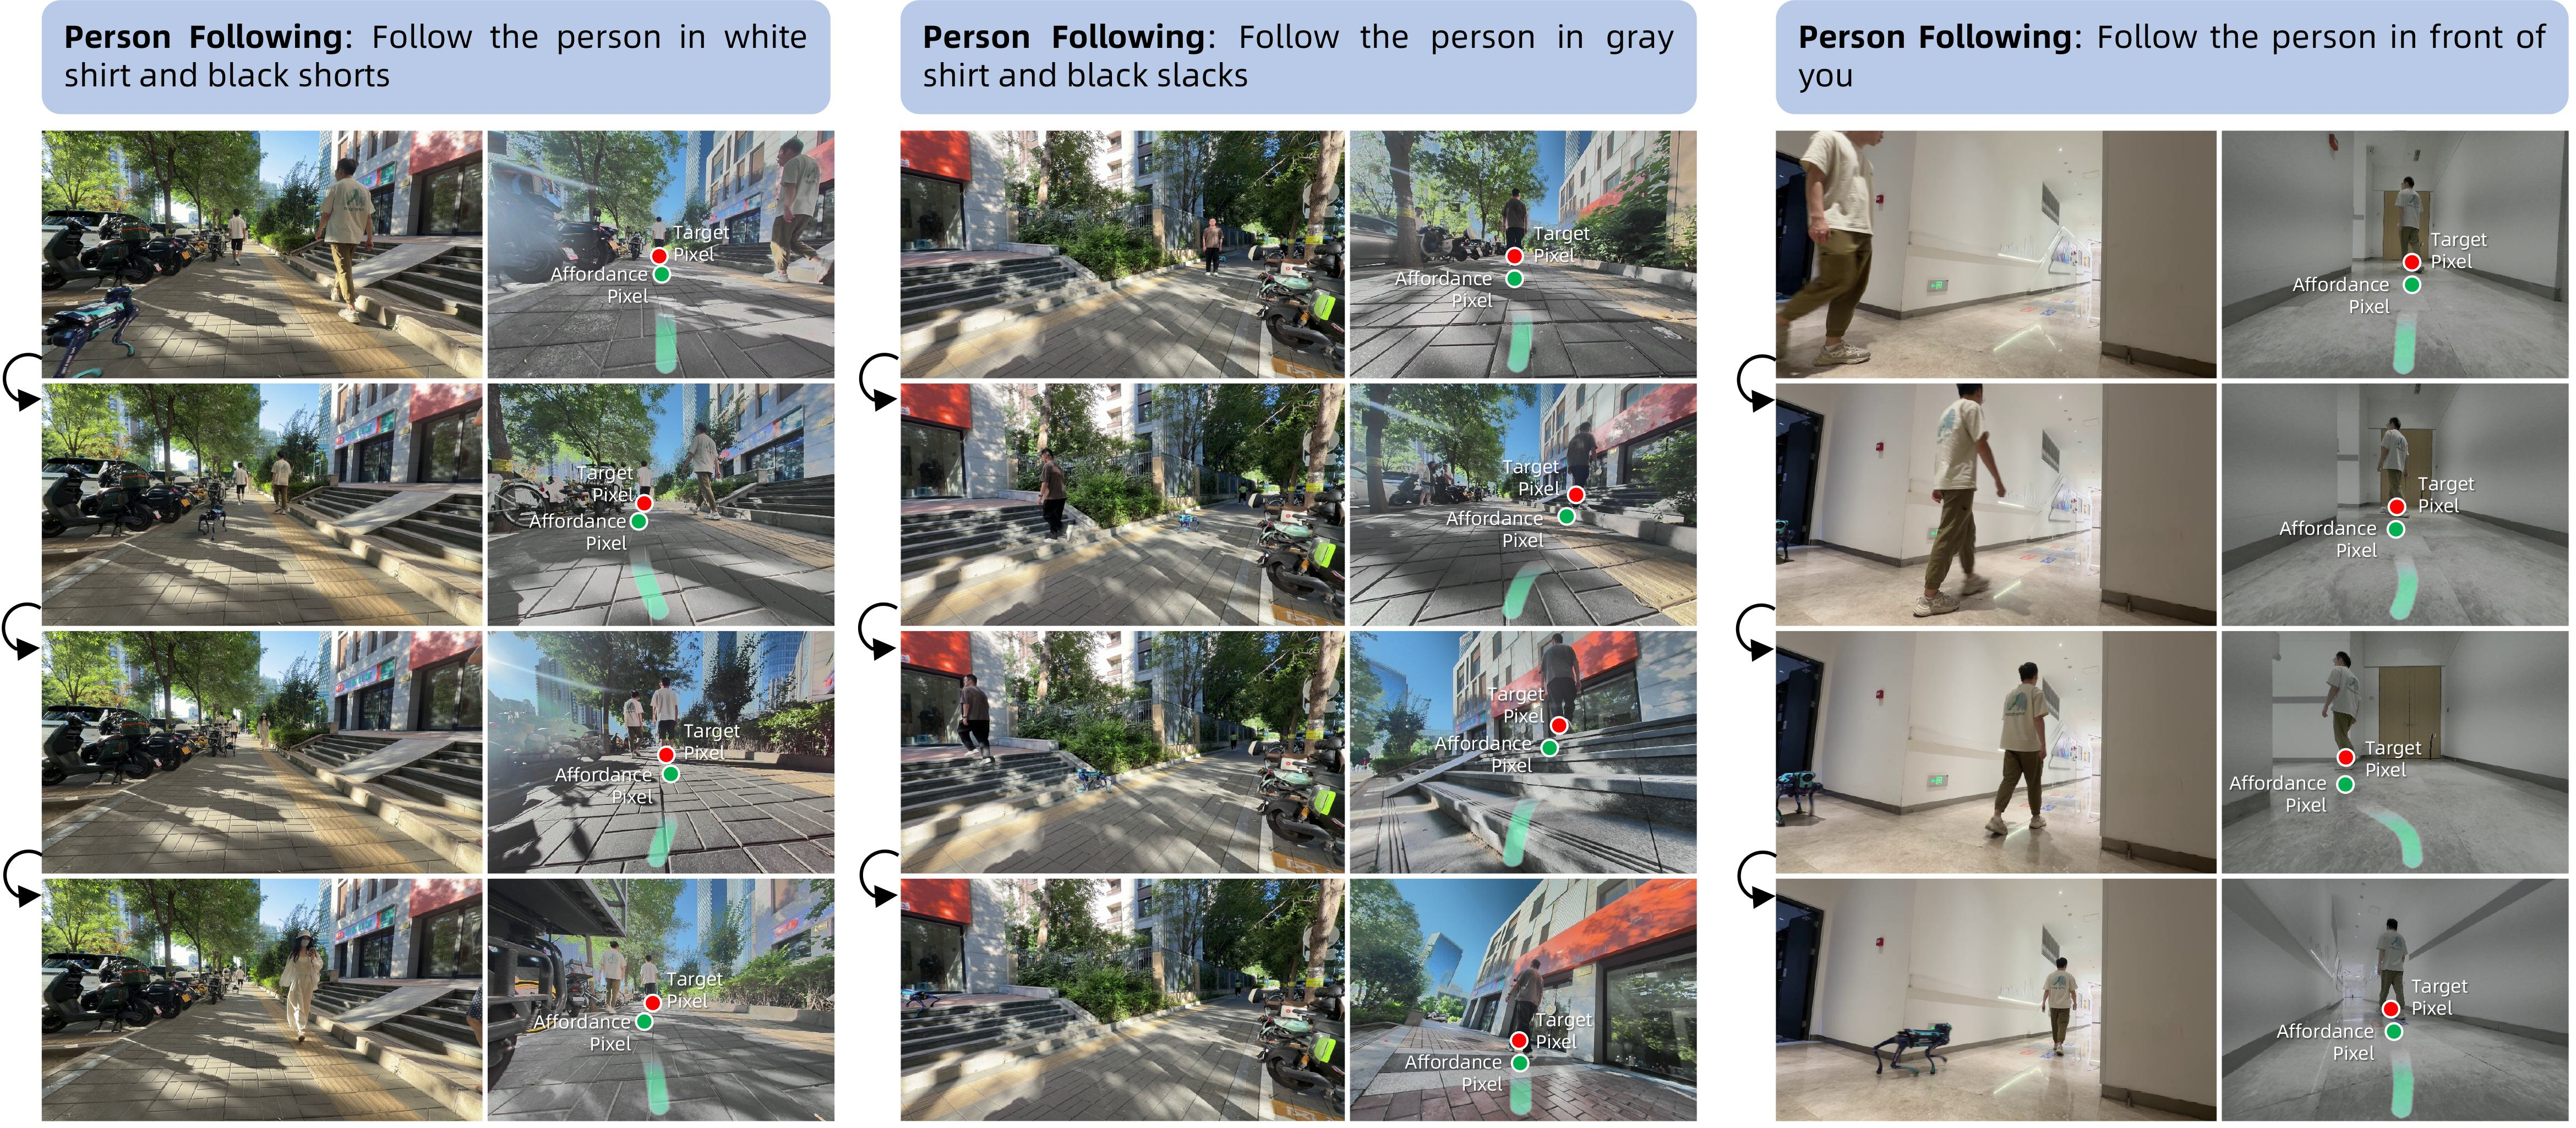
\includegraphics[width=\linewidth]{figs_jpg/person_exp.jpg}

\caption{\textbf{Person-Following Deployment.} Outdoor tracking under
pedestrian distraction, stair-climbing following, and indoor
corner-rounding with temporary occlusion.}
\label{fig:exp-person}
\end{figure}

\paragraph{Summary.}
The five deployment tasks collectively validate the slow-fast
architecture: the slow system provides high-level semantic reasoning---instruction
decomposition, open-vocabulary recognition, spatial relation inference,
rule-aware decision-making, and identity persistence---externalized as
CoT traces and pixel-level grounding; the fast system translates these
pixel anchors into smooth  control with precise last-meter arrival,
dynamic obstacle avoidance, and stable locomotion under terrain variation.
Their asynchronous coupling eliminates odometric drift through
continuous visual re-grounding while the fast system's reactivity
compensates for the slow system's latency, yielding robust,
compliant navigation across all five real-world scenarios.
